
%% begin preamble%%

% set the document class
\documentclass[12pt]{report}

\usepackage[utf8]{inputenc}

% prepare the document for images
\usepackage{graphicx}
% sets the directory where images are stored
\graphicspath{ {images/} }

% set spacing package to change the spacing for the table of contents
\usepackage{setspace}

% package to create captions and subcaptions for figures and tables
\usepackage[labelfont=bf]{caption}
\usepackage{subcaption}

% package to type piecewise functions
\usepackage{amsmath}

% using the geometry package to set margins of the document

\usepackage[a4paper,width=150mm,top=25mm,bottom=25mm]{geometry}


% using packages to add in headers and footers

\usepackage{fancyhdr}
\pagestyle{fancy}

% specifying inputs for headers and footers
\fancyhead{}
\fancyhead[RO,LE]{Thesis Title}
\fancyfoot{}
\fancyfoot[LE,RO]{\thepage}
\fancyfoot[LO,CE]{Chapter \thechapter}

% changing the thickness of the lines in the headers and footers:

\renewcommand{\headrulewidth}{0.4pt}
\renewcommand{\footrulewidth}{0.4pt}

% using the biblatex package to create references


\usepackage[style=apa,sorting=nyt, maxcitenames=2, natbib=true,backend=biber]{biblatex}
\addbibresource{references.bib}

% This allows for an additional line-breaking pass with the amount of "tolerable" white space per line increased by 1em.
\emergencystretch=1em


\title{Thesis Title}
\author{Author Name}
\date{Day Month Year}

%% end preamble%%

\begin{document}

\begin{titlepage}
   \begin{center}
       \vspace*{1cm}
 
       \textbf{ \begin{LARGE}The Application of Machine Learning\\ 
       \vspace{0.3cm} Methods to Time Series Forecasting \end{LARGE}}
 
       \vspace{0.5cm}
        \begin{large} Improving Forecasting Techniques for Smart City Planning \end{large}
 
       \vspace{1.5cm}
 
       \textbf{Authors:}\\
       
       \begin{center}
	  \begin{tabular}{ c c c } 
   \textbf{Manuel Alexander Schreiber}  &  & \textbf{Conor Hasselgard Cavanaugh}\\
	  (676991) &  & (82502)\\ 
	 \end{tabular}
	 \end{center}

	
	   \vspace{0.5cm}        
        
 	  \textbf{Supervisor:} Prof. Lisbeth La Cour, PhD \\
 	  (Department of Economics)
 	  
 	  \vspace{0.5cm}    
 	  
 	  \textbf{Co-Supervisor:} Prof. Raghava Rao Mukkamala, PhD \\
 	  (Department of Digitalization\\ 
 	  and Centre for Business Data Analytics)
 
       \vspace{3cm}
 	
 	A thesis presented for the degrees of a\\
 	     \begin{center}
	  	 \begin{tabular}{ c c c } 
   Master of Science (M.Sc.)  &  & Cand.Merc.Mat (M.Sc.)\\
    in Advanced Economics and Finance &  & in Erhvervsøkonomi og Matematik\\ 
		 \end{tabular}
	 	 \end{center}
	 
 
 
       \vspace{1cm}
 
       
\includegraphics[width=0.4\textwidth]{CBS}
 
       \vspace{1cm}
       
       Number of pages (characters):
       
       Copenhagen Business School\\
       Copenhagen, June 30, 2020
 
   \end{center}
\end{titlepage}

\thispagestyle{plain}
\begin{center}
    \textbf{Abstract}
\end{center}

% type abstract here:

\doublespacing
\tableofcontents
\singlespacing


\listoffigures

\listoftables

% When writing something like a thesis its worth splitting up the document into % multiple .tex files. It's also wise to organise the project using folders;  %therefore, we'll create two new folders, one for all the images used in the %project and one for all the .tex files making up the main body of the thesis.

%\chapter*{Abstract}
%Abstract goes here

\chapter*{Acknowledgements}
I want to thank my supervisor/parents/classmates...

\chapter{Introduction}
Machine learning methods have been developed and refined to the point that they now pose a serious challenge to classic statistical models in the area of forecasting. For example, \citeauthor*{ahmed} \parencite*{ahmed} came up with a large-scale comparison study based on the M3 competition dataset to compare the major machine learning models for time series forecasting. Exponential smoothing models are among the most frequently used forecasting methods. However, \textcite{bergmeir} argue that these models can be substantially outperformed for the purpose of forecasting by applying the bagging algorithm to a bootstrapped component of the initial time series to estimate an ensemble of exponential smoothing models and by combining the resulting point forecasts. 

\section{Preliminary Overview of Relevant Literature}

\citeauthor*{januschowski2020} \parencite*{januschowski2020} provide an overview of the spectrum of Machine learning and statistical methods and the boundaries and intersections in the context of forecasting. This distinction is a common way of classifying forecasting methods in the forecasting literature. However, the authors contend that there is no added value from such a classification of the methods and they encourage the scientific communities to collaborate more.
\textcite{maasoumi2010} present applications in Economics and Finance at the intersection of Statistical Learning and Econometrics. Inter alia, the authors analyze bagging and combination forecasts and find that bagging forecasts often deliver the lowest mean squared forecast errors.

\section{Planned Methodology and Research Design}

As suggested by \textcite{bergmeir}, a Box-Cox transformation can be applied to the series in order to stabilize the variance of the time series and subsequently an STL decomposition is employed to break the time series down into the trend, the seasonal part and the remainder. Bootstrapping the remainder of the series is done to achieve stationarity. Furthermore, \citeauthor*{galicia2019} \parencite*{galicia2019} suggest the use of an ensemble time series forecasting model consisting of three components, which are decision trees, gradient boosted trees and Random Forests. For this model, the ensemble weights are computed by weighted least squares. They found that the ensemble outperforms its individual components. The three ensemble components can thus be employed for the purpose of this paper.



\chapter{Research Questions}
This paper is concerned about the following reseach questions:

\begin{enumerate}
\item[\textbf{(Q1)}] How can forecasting methods be employed to improve city infrastructure planning in a smart city?
\item[\textbf{(Q2)}] What are the best forecasting models for the three Smart City usecases traffic, healthcare and security?
\item[\textbf{(Q3)}] Can the forecasting performance of traditional statistical models for time series forecasting be outperformed or complemented by Machine Learning methods?
\end{enumerate}
 
\chapter{Smart City}
\input{chapters/chapter03}
 
\chapter{Forecasting Methods}
\section{Traditional Statistical models}

\subsection{ARIMA models}

\subsection{Exponential Smoothing models}

\subsection{Holt-Winters models}

\section{Machine Learning Methods}

\subsection{Bagging for Time Series}

According to \textcite{hastie2009} the bagging estimate is defined by

\begin{equation} 
\hat{f}_{bag}(x)=\frac{1}{B} \sum_{b=1}^B\hat{f}^{*b}(x)
\end{equation}

\noindent The bagging estimate is obtained by averaging the predictions $\hat{f}^{*b}(x)$ for\\ $ b=1,..,B $ from the statistical learning models fitted to a collection of B bootstrap samples obtained from the single training data set via taking repeated samples with replacement, i.e. bootstrapping.\\
Bagging is therefore a general-purpose technique for reducing the variance of a statistical learning method, which also increases that method's prediction accuracy \citep{james2013}.\\

\noindent The well-established bagging method was first introduced by \textcite{breiman1996} but it was not successfully applied in a time series forecasting context until 2016.\\
According to \textcite{petropoulos2018} the complication with time series consists in accounting for non-stationarity and autocorrelation in the bootstrapping procedure in order to produce bootstrapped samples that resemble the original data.\\
\textcite{bergmeir} propose a bootstrapping procedure for time series as illustrated in Figure \ref{fig: Bootstrapping procedure TS} that includes a Box-Cox transformation in order to stabilize the variance and a decomposition either in form of the loess method to extract trend and remainder in case of a non-seasonal time series or an STL decomposition in order to break the series down into the trend, seasonal and remainder components. 
The Box-Cox transformation, which was first introduced by \textcite{box1964}, is defined as follows:

\begin{equation}
	w_{t} =
	\begin{cases}
	log(y_{t}), & \lambda=0 \\
	(y_{t}^\lambda-1)/\lambda, & \lambda \neq0\\
	\end{cases}
\end{equation}

The optimal $\lambda \in [0,1]$ is chosen by dividing the series into subseries of length equal to the seasonality and minimzing the coefficient of variation $s/m^{(1-\lambda)}$ across those subseries, where $s$ stands for the standard deviation and $m$ for the sample mean of the subseries.
The authors then apply a bootstrapping method that allows for autocorrelation, the moving block bootstrap (MBB) as suggested by \textcite{kunsch1989}, to the extracted remainder of the series. In the next step, the series is reconstructed from its structural components, i.e. trend, seasonality, and the bootstrapped remainder. Finally, the Box-Cox transformation is inverted. The whole process is then repeated in order to obtain the bootstrapped series.\\ 


\begin{figure} [h]
\centering
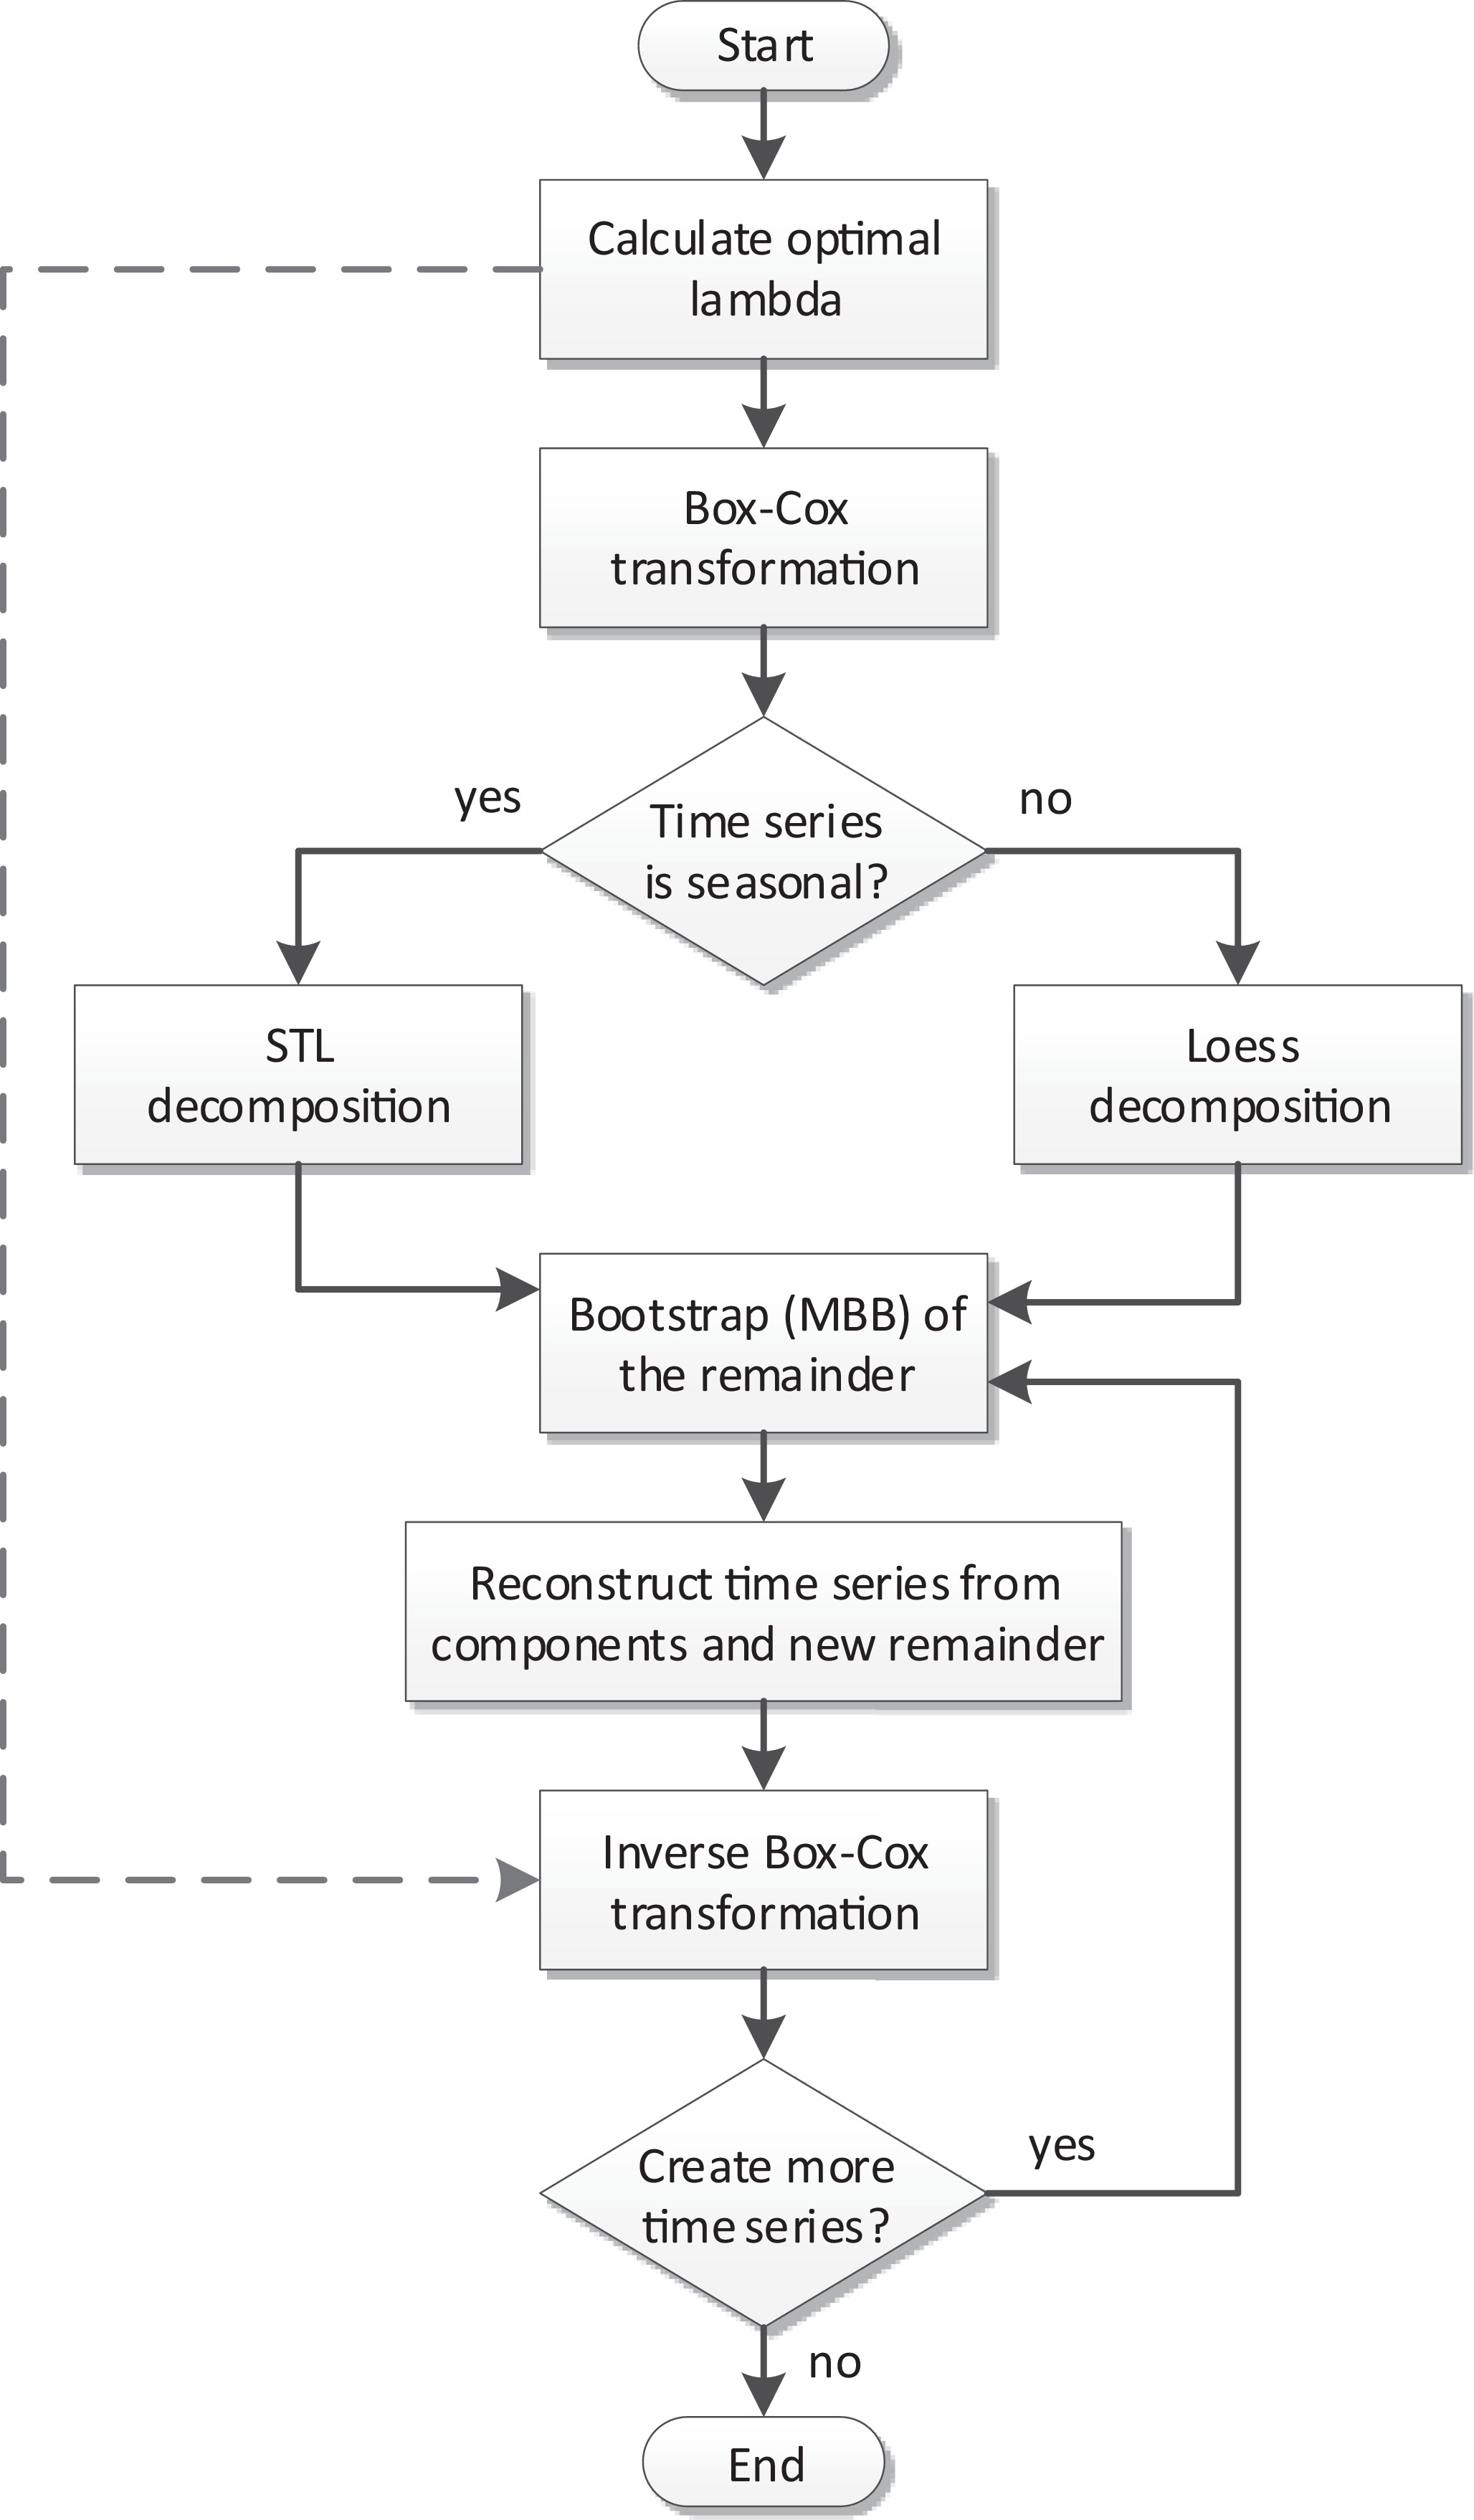
\includegraphics[scale=0.8]{TS}
\caption{Bootstrapping procedure for a time series (adapted from \textcite{petropoulos2018})}
\label{fig: Bootstrapping procedure TS}
\end{figure}

\textcite{bergmeir} find that the ensemble of bagged exponential smoothing models outperforms the regular exponential smoothing model consistently for monthly data on the M3 forecasting competition dataset, which is a common medium of comparison of newly introduced forecasting methods with existing state of the art models.


\subsection{Tree-based models for Time Series}

\textcite{galicia2019} propose a dynamic ensemble model for big data time series forecasting purposes as illustrated in Figure \ref{fig: Dynamic ensemble model} based on the three base models decision trees, random forests and gradient boosted trees. The ensemble weights are computed by weighted least squares assigning higher weights to more accurate ensemble members according to their past performance.\\

 
\noindent The authors found that the ensemble model outperformed the individual base models on a high sampling frequency dataset for the Spanish electricity market in terms of prediction accuracy as evidenced by lower mean absolute errors (MAE) and root mean squared errors (RMSE). Moreover, they found that the dynamic ensemble model could outperform Artificial Neural Network (ANN) and deep learning (DL) algorithms when evaluating forecast errors by yielding the lowest MAE and RMSE values on an Australia solar power dataset.

\begin{figure} [h]
\centering
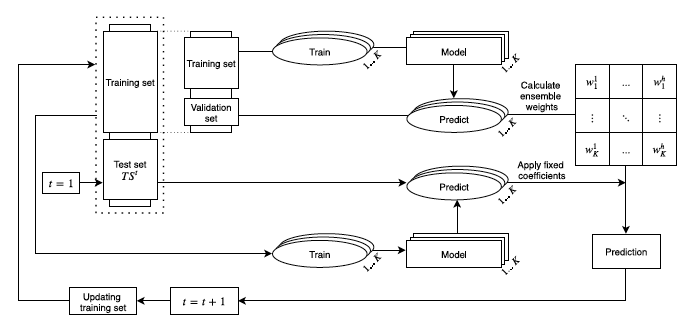
\includegraphics[scale=0.6]{ES}
\caption{Dynamic ensemble model (adapted from \textcite{galicia2019})}
\label{fig: Dynamic ensemble model}
\end{figure}

\subsection{Neural Network Models}

\chapter{Data}
\input{chapters/chapter05}

\chapter{Analyses and Results}
\input{chapters/chapter06}

\chapter{Discussion}
\input{chapters/chapter07}

\chapter{Conclusion}
\input{chapters/conclusion}

\appendix
\chapter{Appendix}
\input{chapters/appendix}

% title option specifies the name of the bibliography
\printbibliography[title = References]


\end{document}

